\documentclass[tikz,border=10pt]{standalone}
\usepackage{pgfplots}
\pgfplotsset{compat=1.18}
\usepgfplotslibrary{fillbetween}

\begin{document}
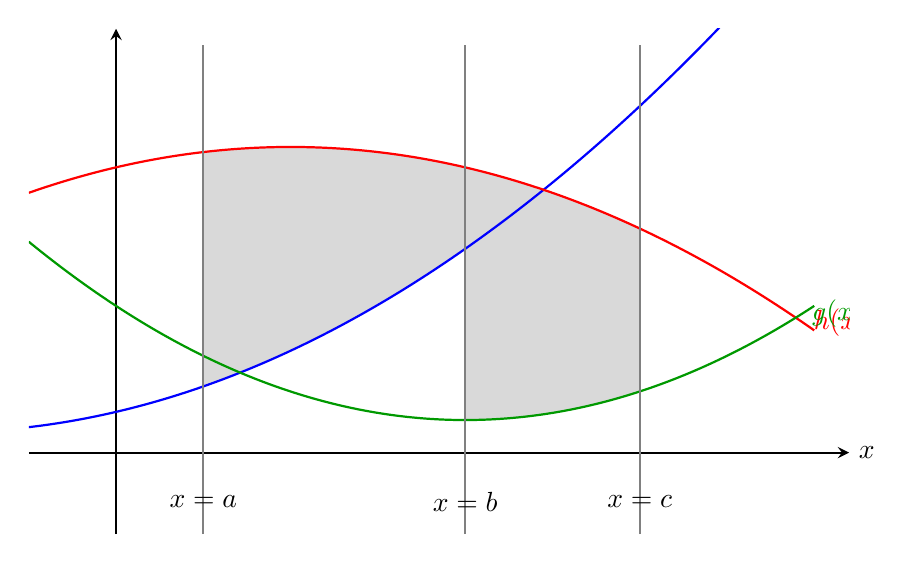
\begin{tikzpicture}
\begin{axis}[
    axis lines=center,
    xlabel={$x$},
    ylabel={},
    domain=-0.5:4,
    samples=200,
    xmin=-0.5, xmax=4.2,
    ymin=-1, ymax=5.2,
    width=12cm,
    height=8cm,
    xtick=\empty,
    ytick=\empty,
    axis line style={-stealth, thick},
    every axis x label/.style={at={(ticklabel* cs:1.0)}, anchor=west},
    every axis y label/.style={at={(ticklabel* cs:1.0)}, anchor=south},
]

% Define the three functions
\addplot[name path=f, blue, thick, domain=-0.5:4, samples=200] {0.25*x^2 + 0.5*x + 0.5} node[right, pos=0.98] {$f(x)$};
\addplot[name path=h, red, thick, domain=-0.5:4, samples=200] {-0.25*x^2 + 0.5*x + 3.5} node[right, pos=0.98] {$h(x)$};
\addplot[name path=g, green!60!black, thick, domain=-0.5:4, samples=200] {0.35*(x-2)^2 + 0.4} node[right, pos=0.98] {$g(x)$};

% Vertical lines at x=a, x=b, x=c
\addplot[gray, thick] coordinates {(0.5, -1) (0.5, 5)};
\addplot[gray, thick] coordinates {(2.0, -1) (2.0, 5)};
\addplot[gray, thick] coordinates {(3.0, -1) (3.0, 5)};

% Labels for vertical lines
\node at (axis cs:0.5, -0.6) {$x=a$};
\node at (axis cs:2.0, -0.6) {$x=b$};
\node at (axis cs:3.0, -0.6) {$x=c$};

% Shaded region between curves
% Region 1: between f and h from x=a to x=b
\addplot[gray, opacity=0.3] fill between[of=f and h, soft clip={domain=0.5:2.0}];

% Region 2: between g and h from x=b to x=c
\addplot[gray, opacity=0.3] fill between[of=g and h, soft clip={domain=2.0:3.0}];

\end{axis}
\end{tikzpicture}
\end{document}
